\documentclass[11pt,a4paper]{article}
\usepackage[margin=1in]{geometry}
\usepackage{graphicx}
\title{Temporal Dynamics of Client Feedback in ERC8004\\Science-Chief Review}
\author{Science-Chief}
\date{2026-03-08}
\begin{document}
\maketitle

\section*{Introduction}
This report studies how client feedback is distributed over time in ERC8004. The target question is behavioral: do some clients produce many feedback events in short bursts and then become inactive, or is issuance mostly stable over time? This distinction matters because temporal concentration can amplify dominance risk even when aggregate counts seem acceptable.

\section*{Data and Method}
The analysis uses feedback events from \texttt{reputation\_newfeedback.csv} (Ethereum ERC8004 reputation registry). Specialist produced block-binned client time series, inter-event gap statistics, lifetime metrics, burst metrics, dropout flags, and behavior labels. SC reviewed these outputs and interprets them here as a unified temporal behavior study.

\section*{Results}
The time-series panel contains 714 client-bin rows across 568 clients and 129 bins. This confirms that activity is sparse in time and concentrated across actors. The lifetime table indicates a median active span of 0 blocks, with a long-tail upper region (p90 around 1,699 blocks), meaning many clients are effectively one-shot while a minority remains active over longer horizons.

Burst diagnostics reinforce the same pattern. Peak-over-average ratios are very high for top actors, and the top burst client reaches a peak window count of 618 events. This is not compatible with a homogeneous, smoothly distributed evaluator base. The cluster output is dominated by the \texttt{whale\_dormant} label, while \texttt{sprinter} is a small minority. Dropout flags are also extremely high (inactive-after-peak rate close to 0.986), which suggests rapid decay after bursts for most clients.

Figure-level reading is coherent with these metrics. The heatmap highlights sparse and uneven temporal occupancy across top clients. The cumulative top-20 trajectories show that a restricted set of clients contributes large shares quickly. The inter-event distribution confirms non-uniform spacing, and the peak-vs-lifetime scatter separates high-intensity short-span behaviors from low-intensity residual activity. The cluster distribution figure summarizes this imbalance explicitly.

\begin{figure}[htbp]
\centering
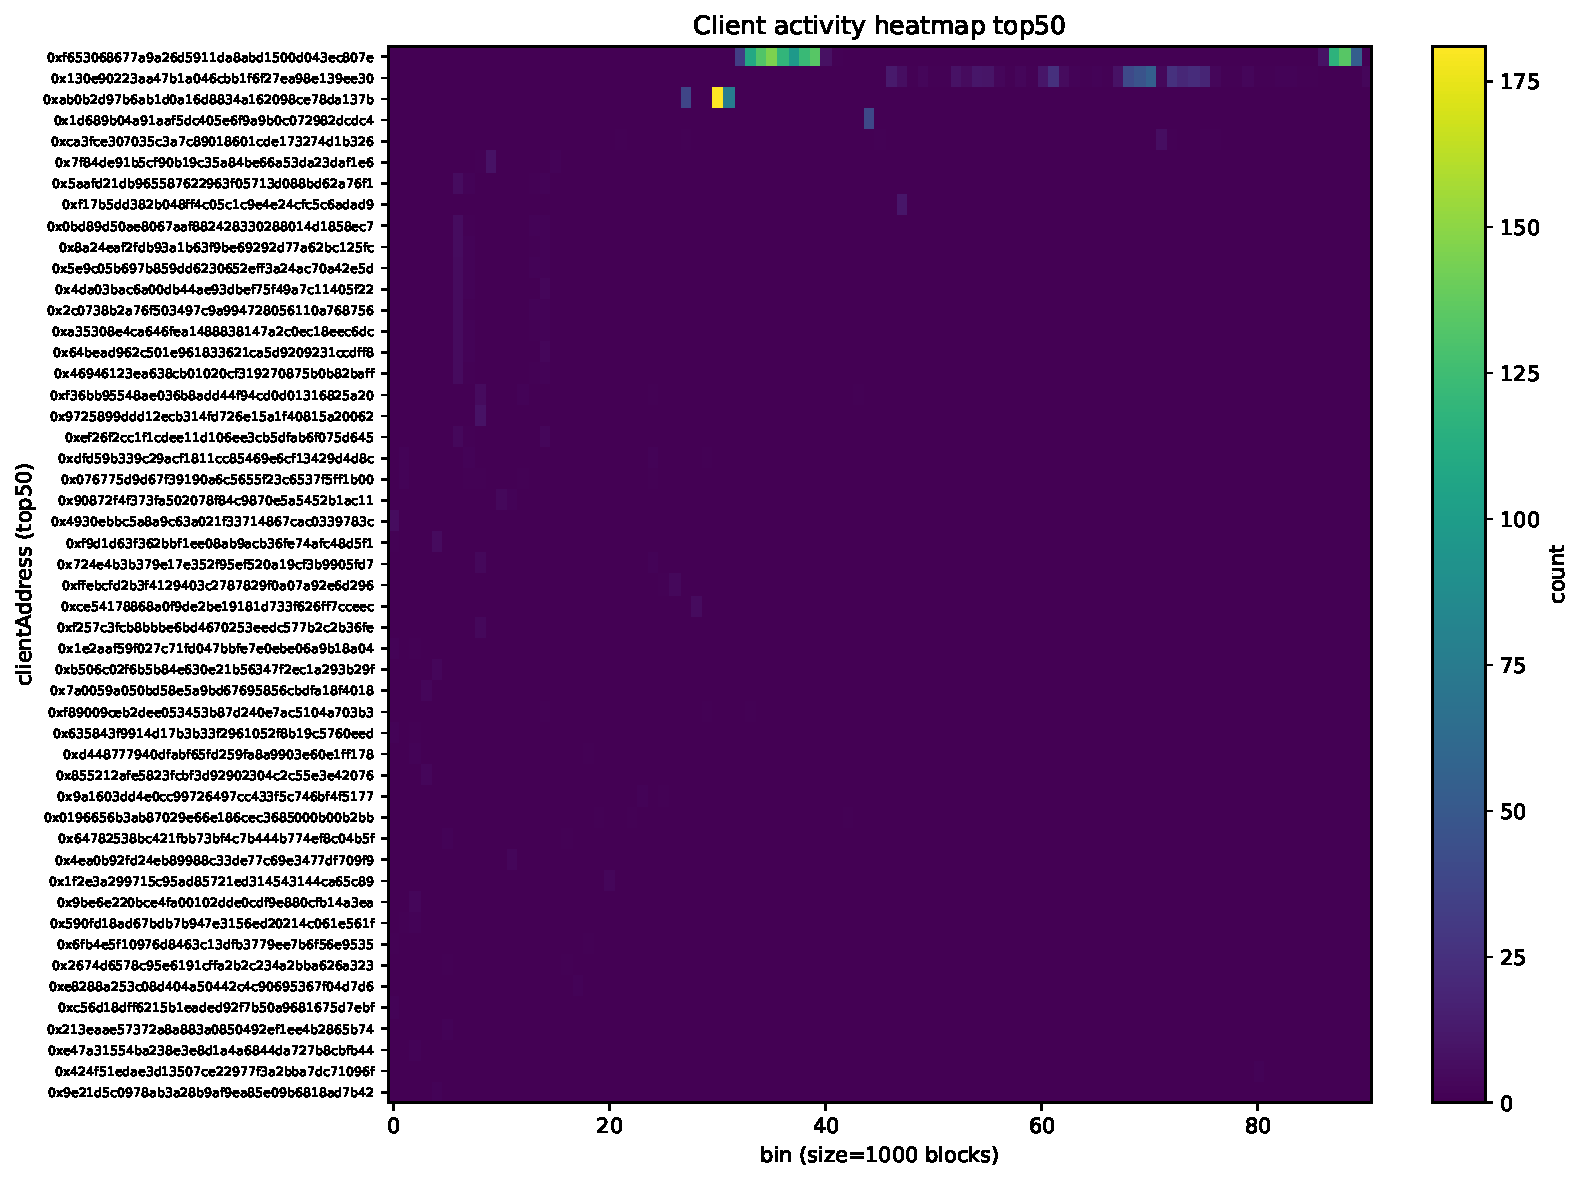
\includegraphics[width=0.86\textwidth]{figures/client_activity_heatmap_top50.pdf}
\caption{Client activity heatmap (top clients).}
\end{figure}

\begin{figure}[htbp]
\centering
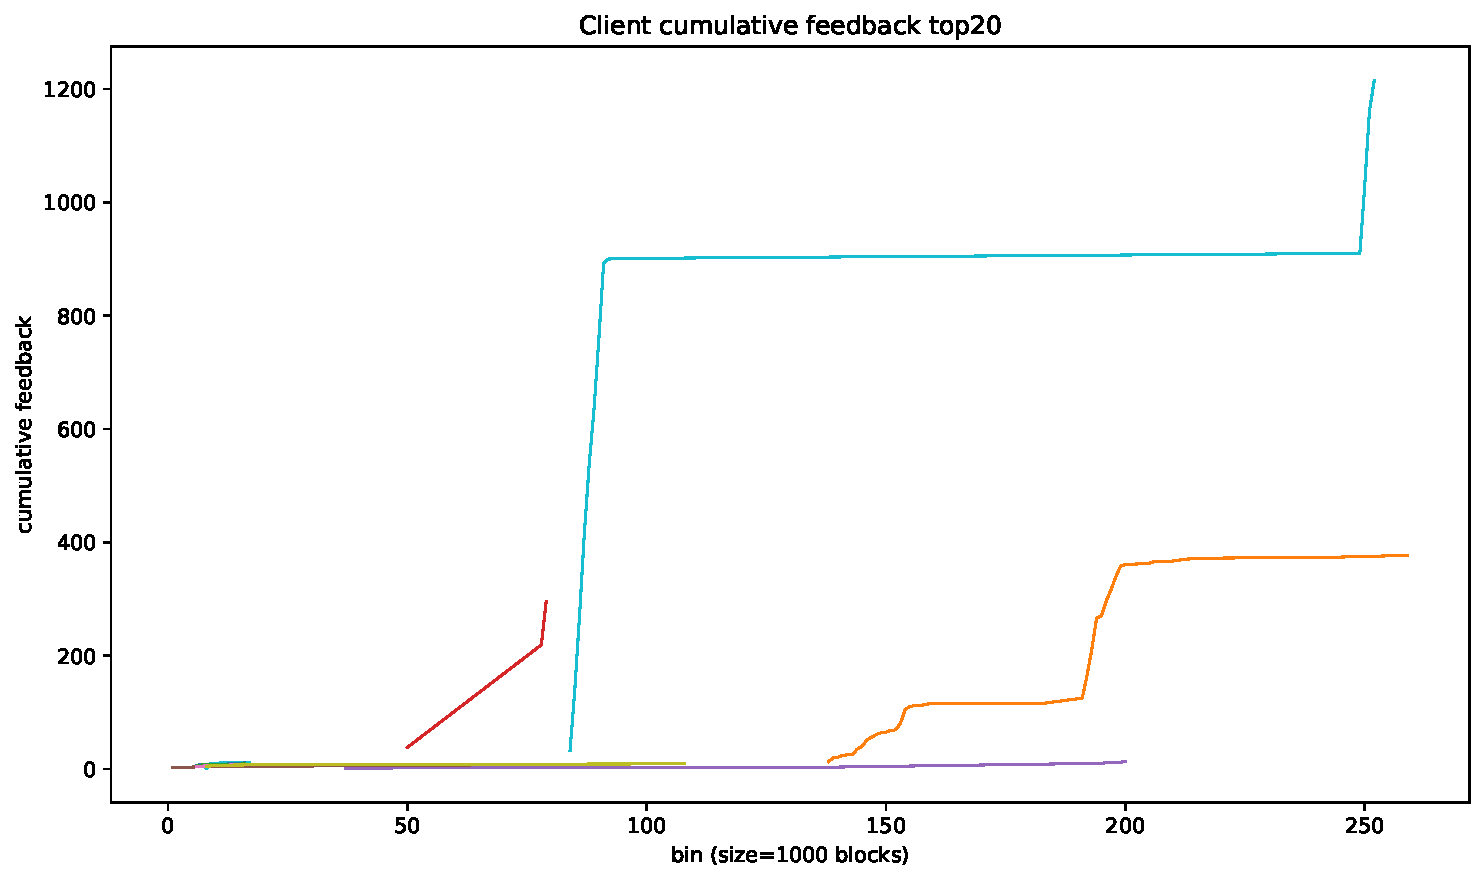
\includegraphics[width=0.86\textwidth]{figures/client_cumulative_feedback_top20.pdf}
\caption{Cumulative feedback trajectories for top clients.}
\end{figure}

\begin{figure}[htbp]
\centering
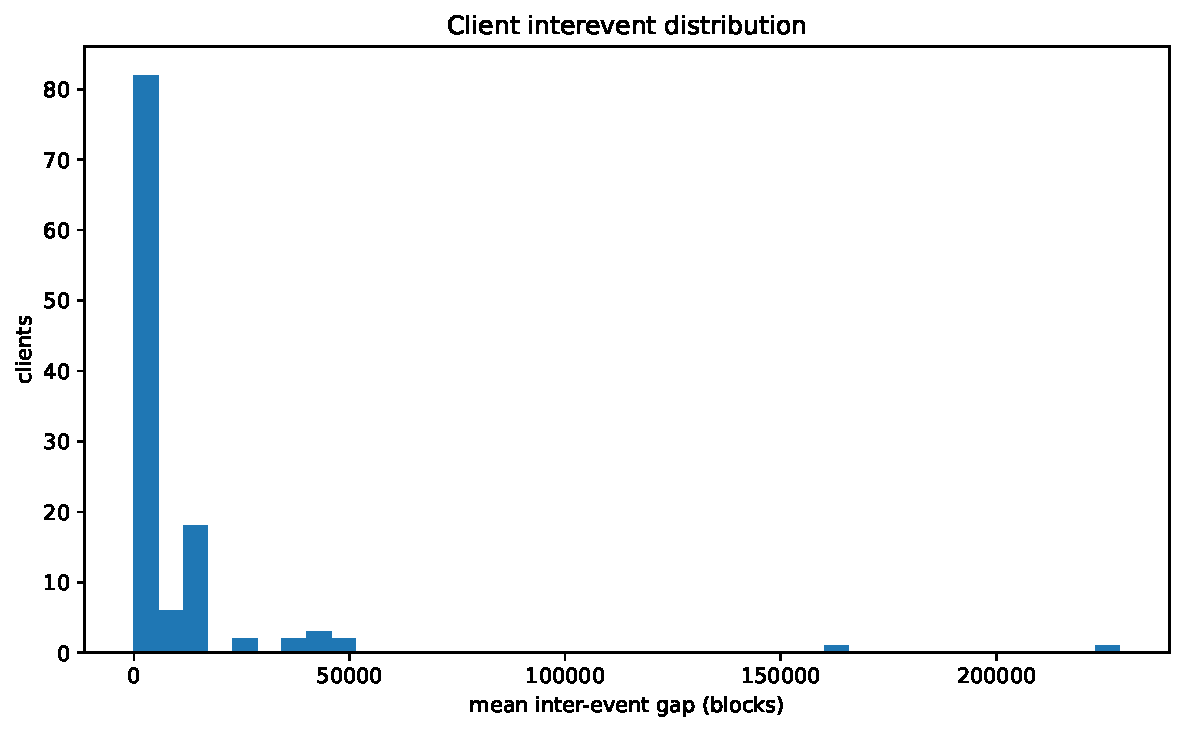
\includegraphics[width=0.82\textwidth]{figures/client_interevent_distribution.pdf}
\caption{Distribution of inter-event behavior.}
\end{figure}

\begin{figure}[htbp]
\centering
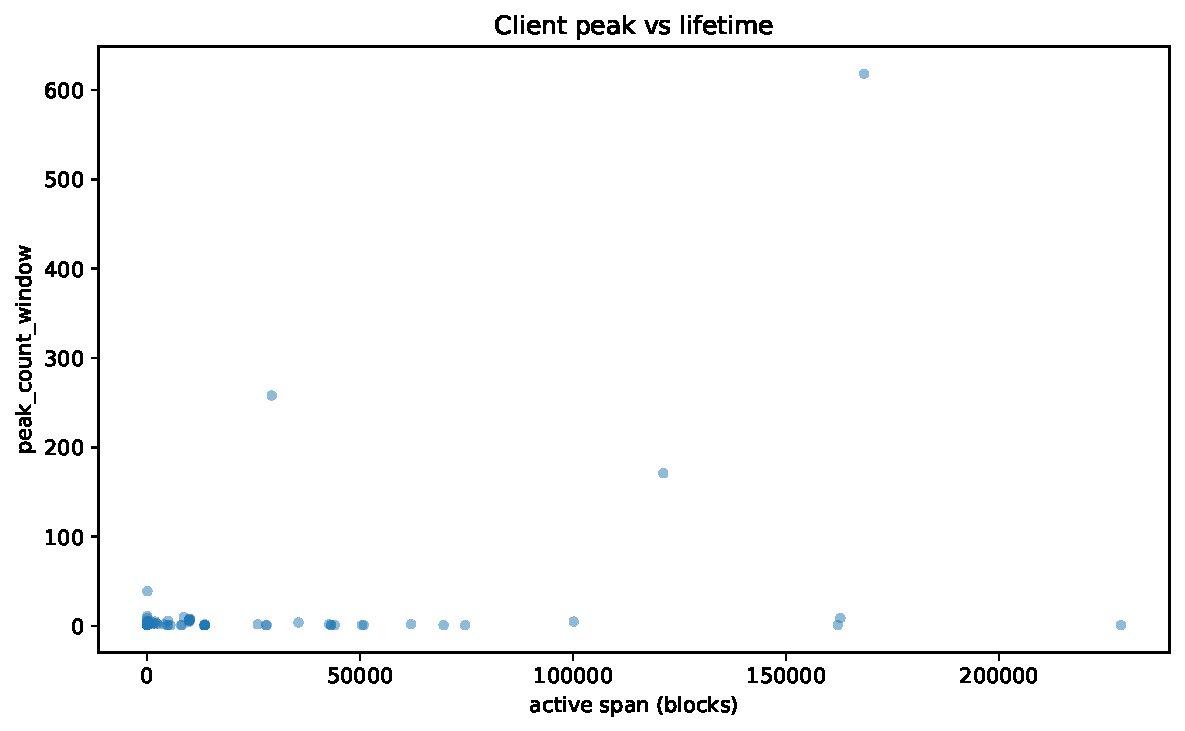
\includegraphics[width=0.82\textwidth]{figures/client_peak_vs_lifetime_scatter.pdf}
\caption{Peak intensity versus active lifetime.}
\end{figure}

\begin{figure}[htbp]
\centering
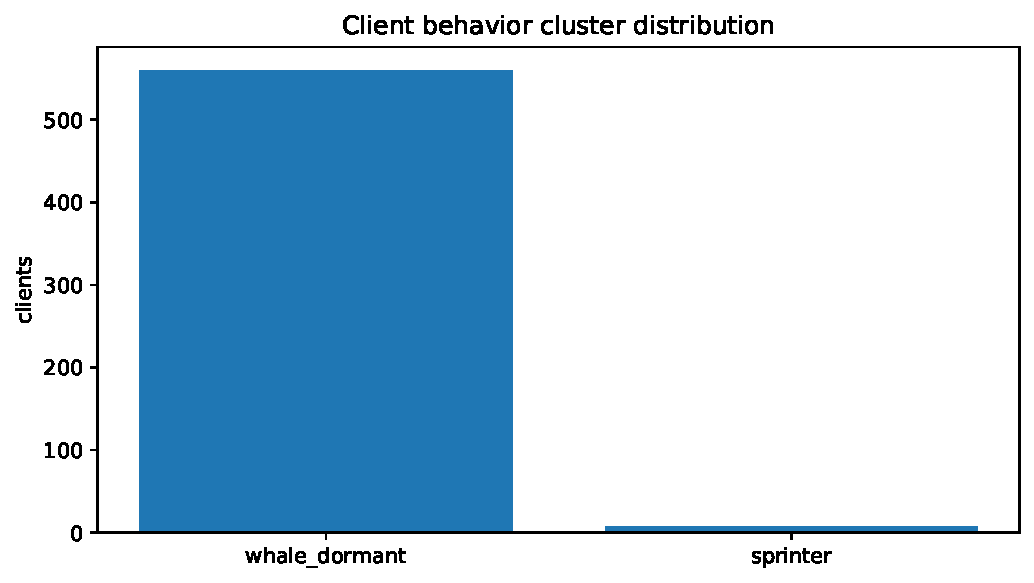
\includegraphics[width=0.75\textwidth]{figures/client_behavior_cluster_distribution.pdf}
\caption{Behavior cluster distribution across clients.}
\end{figure}

\section*{Interpretation}
From a scientific perspective, the temporal layer shows that dominance is not only cross-sectional but also dynamic: high-volume contributions tend to be concentrated in short periods and then decay. In practical terms, this means that the reputation layer can be driven by temporal bursts from a very small evaluator set. Consequently, any interpretation of trust robustness must control for both \emph{who} emits feedback and \emph{when} that emission occurs.

\section*{Limitations}
The current panel is block-time based and Ethereum-only. Some burst metrics appear highly discretized, suggesting that bin-size choices and rule-threshold definitions should be stress-tested. Before external claims, sensitivity analysis on bin width and inactivity thresholds is required.

\section*{Conclusion}
The evidence strongly supports a burst-and-drop temporal regime for client behavior. A minority of clients can emit large bursts and then become inactive, while most clients remain low-intensity or one-shot. Therefore, concentration control in ERC8004 should explicitly include temporal debiasing mechanisms, not only aggregate-share controls.

\section*{Appendix: Source Paths}
\textbf{Figures}\\
\begin{itemize}
\item \texttt{workspaces/science-chief/outbox/Reports/CLIENT\_TEMPORAL\_DYNAMICS\_REVIEW\_2026-03-08/figures/client\_activity\_heatmap\_top50.pdf}
\item \texttt{workspaces/science-chief/outbox/Reports/CLIENT\_TEMPORAL\_DYNAMICS\_REVIEW\_2026-03-08/figures/client\_cumulative\_feedback\_top20.pdf}
\item \texttt{workspaces/science-chief/outbox/Reports/CLIENT\_TEMPORAL\_DYNAMICS\_REVIEW\_2026-03-08/figures/client\_interevent\_distribution.pdf}
\item \texttt{workspaces/science-chief/outbox/Reports/CLIENT\_TEMPORAL\_DYNAMICS\_REVIEW\_2026-03-08/figures/client\_peak\_vs\_lifetime\_scatter.pdf}
\item \texttt{workspaces/science-chief/outbox/Reports/CLIENT\_TEMPORAL\_DYNAMICS\_REVIEW\_2026-03-08/figures/client\_behavior\_cluster\_distribution.pdf}
\end{itemize}

\textbf{Tables}\\
\begin{itemize}
\item \texttt{workspaces/science-chief/outbox/Reports/CLIENT\_TEMPORAL\_DYNAMICS\_REVIEW\_2026-03-08/tables/client\_time\_series\_by\_blockbin.csv}
\item \texttt{workspaces/science-chief/outbox/Reports/CLIENT\_TEMPORAL\_DYNAMICS\_REVIEW\_2026-03-08/tables/client\_interevent\_stats.csv}
\item \texttt{workspaces/science-chief/outbox/Reports/CLIENT\_TEMPORAL\_DYNAMICS\_REVIEW\_2026-03-08/tables/client\_lifetime\_stats.csv}
\item \texttt{workspaces/science-chief/outbox/Reports/CLIENT\_TEMPORAL\_DYNAMICS\_REVIEW\_2026-03-08/tables/client\_burst\_metrics.csv}
\item \texttt{workspaces/science-chief/outbox/Reports/CLIENT\_TEMPORAL\_DYNAMICS\_REVIEW\_2026-03-08/tables/client\_behavior\_clusters.csv}
\item \texttt{workspaces/science-chief/outbox/Reports/CLIENT\_TEMPORAL\_DYNAMICS\_REVIEW\_2026-03-08/tables/client\_dropout\_flags.csv}
\end{itemize}

\end{document}
